\subsection{WebsocketServer}
Die Klasse \eigenName{WebsocketServer} 
%kurze Erwähnung sinn der klasse
%datenaustausch zwischen WebsocketServer zu abgeleitetrer...(dispatcher.... ) (I/O)
\begin{figure}[ht]
  \centering
  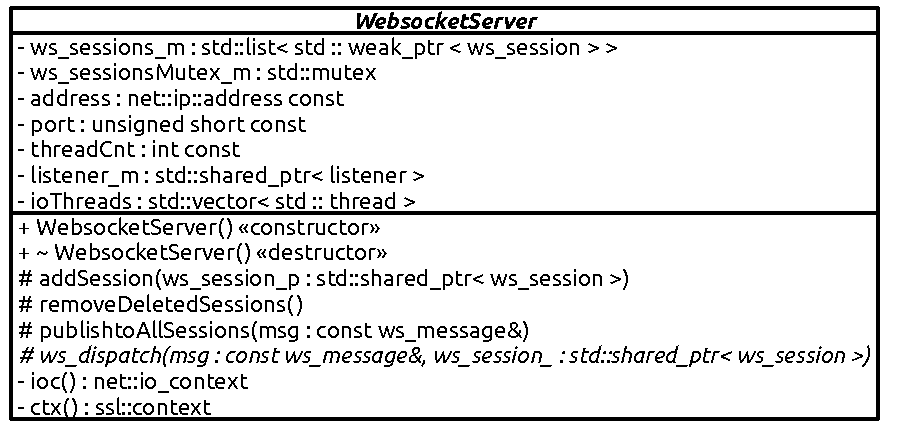
\includegraphics[width=\textwidth]{content/hauptteil/umsetzungPoC/backend/uml/classesOfOverview/WebsocketServer.pdf}
  \caption{Klassediagramm der Klasse \eigenName{WebsocketServer}}
  \label{fig:backend:classDiag:WebsocketServer}
\end{figure}
%beschreibung msg klasse mit diagram
\begin{figure}[ht]
  \centering
  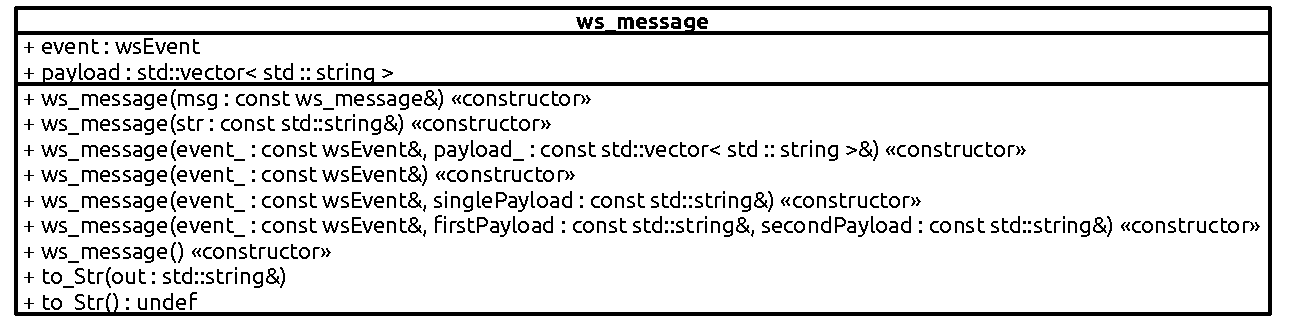
\includegraphics[width=\textwidth]{content/hauptteil/umsetzungPoC/backend/uml/classesOfOverview/ws_message.pdf}
  \caption{Klassediagramm der Klasse \eigenName{ws\_message}}
  \label{fig:backend:classDiag:wsMsg}
\end{figure}
%dispatcher codeausschnitt
%beschreibung dispatcher